\chapter{Context}\label{context}
\section{Use case: TU Delft (working title)}
% Matthijs
% Information about location
This projects main area of interest is the campus of the TU Delft. There are more than 20.000 students using the campus on more than 150 hectares. This emphasises even more the magnitude of this project. The network logs the devices connected to the eduroam access points, which implicitly means logging the (approximate) location of the person carrying the device and more information. This tracking data can be used to derive information about the personality of the person carrying the device, such as the distinction between staff and students, based on the tracked locations. Connection to the Wi-Fi eduroam network is free of charge and requires only a NetID, which all students and staff get upon registration at the university. \\\\
It is very important to understand, that 'no data is also data'. This means that a devices that is not being tracked by any access point for a period of time, is either off-campus or disconnected and still on campus. This provides valuable information when researching the movement patterns. This will be further discussed in the \autoref{preprocessing}. \\\\
The eduroam network of the TU Delft campus consists of 1730 access points, distributed over more than 30 buildings. The data is collected for each of the access points over a period of little more than 3 months. The logs are stored in a database on a virtual server, where it is accessible to the three project groups and the Geomatics staff. The data that is collected and the storage in the database is further described in \autoref{datadescription}. \\\\
The department of Facility Management and Real Estate (FMRE) is the main client for the entire Synthesis Project. They would like to know how the campus is being used, what the hotspots on campus and in buildings are, when people travel the most from one building to another and which buildings are most visited.

\section{Previous research: Rhythm of the campus}
% Matthijs
% Summary of their summary
In the fall of 2014, similar research was conducted during another edition of the Geomatics Synthesis Project. The group "Rhythm of the campus" investigated the use of the Library and the Aula of the TU Delft, to gain insight in patterns the use of the facilities of the Library and Aula. This section will give a short summary of their research (\cite{rhythmofthecampus}).\\\\
During the project, the group used passive Wi-Fi monitoring to detect users of the TU Delft Library and the Aula to gain insight in the occupation, in request of FMRE. They used BlueMark sensors at the Library, Aula and 5 other faculties for a period of one week and collected ground truth data for 2 days. Due to its sheer size, the raw data was difficult to process. The data was filtered from static devices and outliers and the data analysis resulted in identification of the occupation of the Library and the Aula. The end results was a dashboard which visualized the sensor network, data analysis and pattern recognition to help the client in the decision making process.\\\\
This research was different from the research conducted in this Synthesis Project, mainly due the larger size of the eduroam network and the ability to track everybody using the Wi-Fi network.

\section{Privacy}
This project focuses on identifying common movement patterns, ignoring the individual, therefore we did not test explicitly whether is possible to identify individuals or not from the data. However, based on our findings about the operation of the \textit{eduroam} Wi-Fi network and about the methods that
are used to identify movement patterns, we can make the following assumptions.\\\\
Movement patterns are rather unique, therefore it is possible to match them to individuals even if maybe not in every case. However, in order to do so it is
necessary to have additional data available. This additional data itself is often considered private data, e.g. the complete weekly schedule of the person.
Provided that timetables are openly accessible and the occupation of the individual is known, then his movement pattern may be identified in the dataset.\\\\
The availability of a detailed access point map makes it easier to identify individuals by allowing a more detailed movement analysis (e.g. on buildingpart
level). It reduces the ambiguity that is still present in building level movement analysis.

\section{Data accuracy}
The spatial accuracy of the Wi-Fi log datased is defined by the range of the
APs. Although we do not have information on the exact range of the differente
APs, we estimate the range ot be a few tens of meters. Therefore, if a user is
recorded by a specifis AP, in reality he can be anywhere around the AP in its
range.

The temporal accuracy of the Wi-Fi log dataset is defined by the five minute
campus-wide scan interval of the \textit{eduroam} system. It means that all APs
on the TU Delf campus scan at the same moment in approximately five minute
intervals. Therefore, it is possible that the user is already at a given AP, but
he will be first recorded at the next scan round, or the user alread left the AP
but that also will be only recorded at the next scan round.

\section{Representativeness}
% Xander
In the GSP a big amount of wifilog data is used. The data represents all people that make (active) use of the wifi eduroam network. These are the students and employees of the TU Delft.  There is just a small amount of people that are within the spatial scope of the project and cannot connect with the wifi eduroam network. The data is acquired by the access points, which all are located in a building on the campus. The people that use a building on the campus, but do not make use of the wifi eduroam network, is very small part. Thus, the main part of actual users is covered by the data used in the GSP. The collection of data is acquired over a continuous time interval of more than 2 months. This time period would be large enough to reflect on all users of the campus to some extend.
\section{Data description and System of APs}\label{datadescriptionandsystemofaps}
\subsection{Data description}\label{datadescription}
This section will describe the main datasource used within the Geomatics Synthesis Project; a PostgreSQL database containing the logs from the Wi-Fi access points on the TU Delft campus. The wifilog table has several column, with a data value for each row (\autoref{segmentwifilog}).\\\\
\begin{table}[H]
	\centering
	\captionsetup{justification=centering}
	\caption{A segment of the main datasource; the wifilog table}
	\label{segmentwifilog}
	\begin{tabular}{@{}lllllllll@{}}
		\toprule
		\textbf{username} & \textbf{mac} & \textbf{asstime} & \textbf{apname}  & \textbf{maploc}                                                     & \textbf{sesdur} & \textbf{snr} & \textbf{ssi}          \\ \midrule
		j85cCQ..      & l6iOu+.. & 14-4-2016 12:30  & A-23-0-029 & ..CITG \textgreater 4e Verdieping       & 1:32:02         & 35           & -57\\
		wrBqM..       & f2Pw/P.. & 14-4-2016 7:49   & A-23-0-035 & ..CITG \textgreater 5e \& 6e Verdieping & 5:32:16         & 37           & -56\\
		wrBqM..       & f2Pw/P.. & 14-4-2016 13:22  & A-23-0-035 & ..CITG \textgreater 5e \& 6e Verdieping & 0:40:20         & 46           & -50\\
		wrBqM..       & f2Pw/P.. & 14-4-2016 14:02  & A-23-0-093 & ..CITG \textgreater 5e \& 6e Verdieping & 1:27:13         & 11           & -86\\
		wrBqM..       & f2Pw/P.. & 14-4-2016 15:29  & A-23-0-091 & ..CITG \textgreater 5e \& 6e Verdieping & 0:05:08         & 30           & -65\\
		wrBqM..       & f2Pw/P.. & 14-4-2016 15:34  & A-23-0-035 & ..CITG \textgreater 5e \& 6e Verdieping & 1:42:32         & 29           & -65\\
		J0IwA+..      & HkLY1U.. & 14-4-2016 11:33  & A-23-0-035 & ..CITG \textgreater 5e \& 6e Verdieping & 1:27:40         & 33           & -59\\
		J0IwA+..      & HkLY1U.. & 14-4-2016 13:01  & A-23-0-035 & ..CITG \textgreater 5e \& 6e Verdieping & 1:01:01         & 26           & -68\\
		J0IwA+..      & HkLY1U.. & 14-4-2016 14:02  & A-23-0-035 & ..CITG \textgreater 5e \& 6e Verdieping & 3:30:19         & 25           & -68\\
		J0IwA+..      & HkLY1U.. & 14-4-2016 17:32  & A-23-0-035 & ..CITG \textgreater 5e \& 6e Verdieping & 0:40:05         & 27           & -69\\ \bottomrule
	\end{tabular}
\end{table}
The data value for each attribute (column) in the wifilog table will be described in more detail.\\\\
\textbf{Username}\\
The username column provides the username, as a hashed text. Every user has a unique username, but can appear in the data more than once.
\\\\
\textbf{Mac}\\
The mac column provides the media access control adress (MAC address), as a hashed text. The MAC address is a unique identifier assigned to a specific piece of hardware, such as the network adapter located in Wi-Fi devices (mobile phones, tablets, laptops etc.). So, it would be possible that a user can have more than one device connected to the Wi-Fi eduroam network at the same time.
\\\\
\textbf{Asstime}\\
The asstime is the time of which a connected device is recorded by the system.
\\\\
\textbf{Apname}\\
The apname is the name assigned to the access point. Every access point has a unique name. 
\\\\
\textbf{Maploc}\\
The maploc describes the location of the access point. There could be multiple access points with the same maploc. For instance, there are 31 access points located on the ground floor of the Faculty of Architecture.\\
\begin{figure}[H]
	\centering
	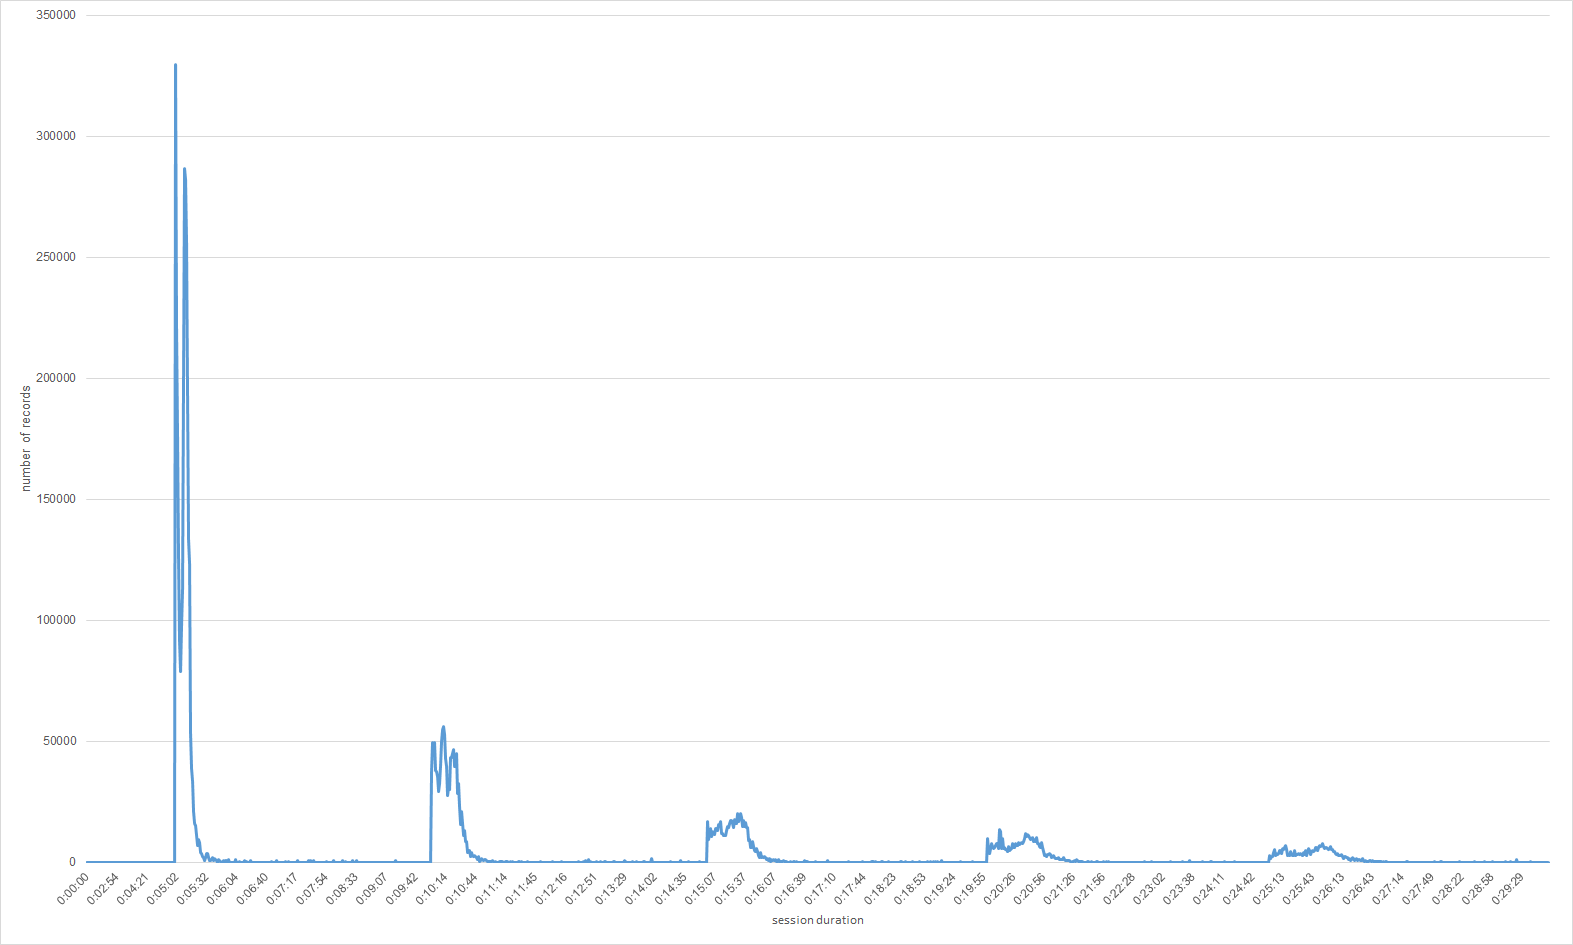
\includegraphics[scale=0.15]{sesdur_graph_without5min.png}
	\captionsetup{justification=centering}
	\caption{The frequency of session durations}
	\label{frequency_sesdur}
\end{figure}
\textbf{Sesdur}\\
The sesdur describes the session duration of which a device is connected to the access point. Because this is not as straightforward as it seems, this will be explained more extensively. \autoref{frequency_sesdur} shows the frequency of session durations (the peak at exactly 5 minutes is filtered out to make the graph more readable). There is a large peak at exactly 5 minutes, a peak at approximately 5 minutes and decreasing peaks after a time interval of approximately 5 minutes. It looks like it is recording in a certain time interval in which the device is (still) connected. \\\\
In order to justify this, the query below is used to see the asstimes (and time to next asstime)\\\\
\begin{center}
\begin{lstlisting}[language=SQL]
select *, asstime_next-asstime as difference
from (
	select count(*),asstime, lead(asstime) over (order by asstime) asstime_next
	from wifilog
	where extract(day from asstime) = 4
	and extract(month from asstime) = 4
	and extract(year from asstime) = 2016
	group by asstime
	order by asstime) as subquery
\end{lstlisting}
\end{center}
\begin{table}[H]
	\centering
	\captionsetup{justification=centering}
	\caption{The time and time to next scan at a random day}
	\label{timetonextscan}
	\begin{tabular}{@{}llll@{}}
		\toprule
		count & asstime        & asstime\_next  & difference \\ \midrule
		2578  & 4-4-2016 13:04 & 4-4-2016 13:09 & 0:05:10    \\
		2435  & 4-4-2016 13:09 & 4-4-2016 13:15 & 0:05:11    \\
		2486  & 4-4-2016 13:15 & 4-4-2016 13:20 & 0:05:11    \\
		2530  & 4-4-2016 13:20 & 4-4-2016 13:25 & 0:05:11    \\
		2471  & 4-4-2016 13:25 & 4-4-2016 13:30 & 0:05:11    \\
		2444  & 4-4-2016 13:30 & 4-4-2016 13:35 & 0:05:11    \\
		2524  & 4-4-2016 13:35 & 4-4-2016 13:40 & 0:05:11    \\
		2588  & 4-4-2016 13:40 & 4-4-2016 13:46 & 0:05:12    \\
		2690  & 4-4-2016 13:46 & 4-4-2016 13:51 & 0:05:11    \\
		2560  & 4-4-2016 13:51 & 4-4-2016 13:56 & 0:05:11    \\ \bottomrule
	\end{tabular}
\end{table}
\autoref{timetonextscan} shows that the time to the next scan is 5 minutes and several seconds in all cases. Most important is to know that all access points are recording the connected device(s) is at the same time. \\\\                                                       
\autoref{sesdur_example} will be used to explain the way the time interval of approximately 5 minutes is coming back in the session duration.\\\\
The first record shows the device is not connected to any of the access points on the campus in the subsequent moment of recording, resulting in a session duration of exactly 5 minutes. The last record in \autoref{sesdur_example} shows the result of a device that is still connected to the same access point at the subsequent moment of recording. In this case the session duration will be 10 minutes and 21 seconds. This is the time interval between the first moment the device is recorded and the first time the device is not recorded by the same access point anymore. The record with id number 6 describes a situation in which the device is connected to an access point at the moment of recording and connected to another access point at the subsequent moment of recording, the session duration is 5 minutes and 18 seconds in this case. This is the time interval between the two moments of recording. This time interval can vary, but is always approximately 5 minutes.\\\\
\begin{table}[H]
	\centering
	\captionsetup{justification=centering}
	\caption{Varying session durations}
	\label{sesdur_example}
	\begin{tabular}{@{}lllllll@{}}
		\toprule
		\textbf{id} & \textbf{username} & \textbf{mac} & \textbf{asstime} & \textbf{apname} & \textbf{maploc}                                                                     & \textbf{sesdur} \\ \midrule
		1           & oHh0Sz..      & WWW0Cd.. & 1-4-2016 10:13   & A-12-0-104      & ..\& Proeffabriek \textgreater !e Verdieping                 & 0:05:00         \\
		2           & oHh0Sz..      & WWW0Cd.. & 1-4-2016 10:18   & A-132-0-064     & ..32-OCP-IO \textgreater 1e Verdieping                     & 0:20:27         \\
		3           & oHh0Sz..      & WWW0Cd.. & 1-4-2016 11:36   & A-132-0-105     & Root Area                                                                           & 0:15:22         \\
		4           & oHh0Sz..      & WWW0Cd.. & 1-4-2016 11:51   & A-132-0-066     & ..32-OCP-IO \textgreater 1e Verdieping                     & 0:20:35         \\
		5           & oHh0Sz..      & WWW0Cd.. & 1-4-2016 14:01   & A-132-0-069     & ..32-OCP-IO \textgreater 1e Verdieping                     & 0:05:43         \\
		6           & oHh0Sz..      & WWW0Cd.. & 1-4-2016 14:06   & A-132-0-133     & ..32-OCP-IO \textgreater 4e Verdieping                     & 0:05:18         \\
		7           & oHh0Sz..      & WWW0Cd.. & 1-4-2016 14:12   & A-132-0-066     & ..32-OCP-IO \textgreater 1e Verdieping                     & 0:05:10         \\
		8           & oHh0Sz..      & WWW0Cd.. & 1-4-2016 14:17   & A-132-0-104     & ..32-OCP-IO \textgreater 2e Verdieping                     & 0:05:10         \\
		9           & oHh0Sz..      & WWW0Cd.. & 1-4-2016 14:22   & A-132-0-067     & ..32-OCP-IO \textgreater 1e Verdieping                     & 0:05:10         \\
		10          & oHh0Sz..      & WWW0Cd.. & 1-4-2016 14:27   & A-132-0-066     & ..32-OCP-IO \textgreater 1e Verdieping                     & 0:10:21         \\ \bottomrule
	\end{tabular}
\end{table}
\textbf{SNR}\\
The signal to noise ratio(SNR) describes a measurement that compares the signal strength to the level of background noise (in dB).\\\\
\textbf{RSSI} \\
The received signal strength indicator (RSSI) describes the received signal strength (in dB).

\subsection{System of APs}\label{systemofaps}
This section will describe the current layout of access points (APs) on the TU Delft campus. The location of APs in a building is not known, but for the Faculty of Architecture a paper map was available. Therefore the system of APs in the Faculty of Architecure will be described in more detail. \\\\
In total there are 1730 access points, distributed over more than 30 buildings on the campus. The access points are mostly placed on walls or ceilings. The data describes that every access point is linked to a certain location. Due to the (wide) signal range of the access point, the device can be located at a different floor level than the access point it is connected to. Moreover, there could be access points located at the first floor while serving people at ground floor as well. This is the case in rooms with high ceilings, such as the orange hall in the Faculty of Architecture. \\\\
As said, the Faculty of Architecure is the only building of which the location of the access points are known. The floor plans are enriched with the location of the access point (see ). Next to that, a table is provdided with additional information regarding the access points, although this table does not contain all present access points. This table includes the MAC address of the access point. This could be used to look up to what access point the device is connected.\\\\
\begin{figure}[H]
	\centering
	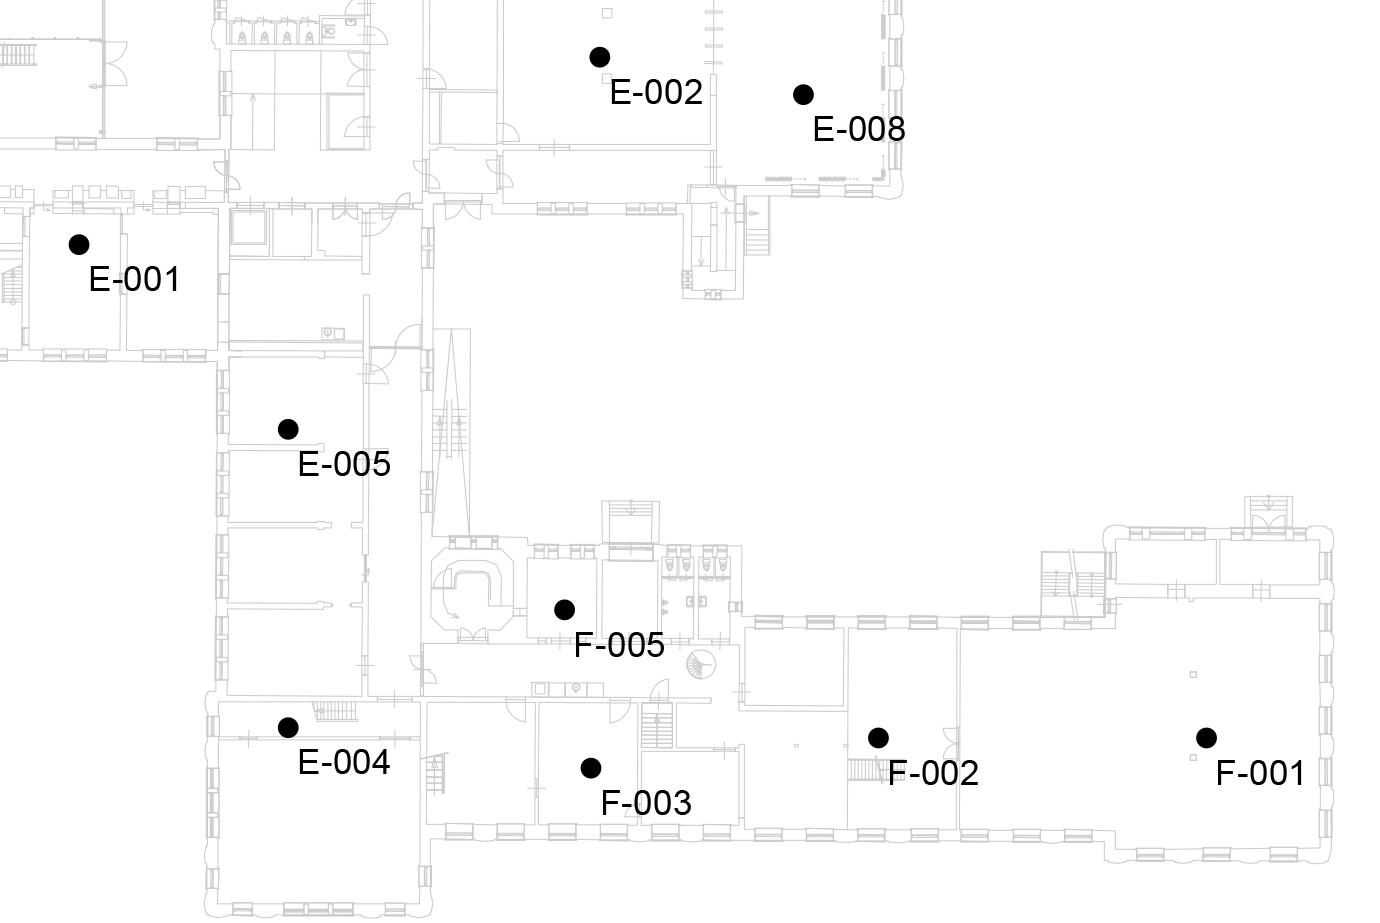
\includegraphics[scale=0.6]{apmap_west.png}
	\captionsetup{justification=centering}
	\caption{Ground floor plan with the location of the access points}
	\label{apmap_west}
\end{figure}

